\documentclass[12pt]{article}

\usepackage[margin=1in]{geometry}
\usepackage{amsmath,amsthm,amssymb}
\usepackage{fancyhdr}
\usepackage[small,compact]{titlesec}
\usepackage{float}

\lhead{Erich Menge}
\chead{\classnameandsection}
\rhead{\homeworktitle}

\pagestyle{fancy}

\newcommand{\sethomeworknumber}[1]{
  \newcommand{\homeworktitle}{Homework #1}
}

\newcommand{\N}{\mathbb{N}}
\newcommand{\Z}{\mathbb{Z}}
\newcommand{\homeworkheader}[1]{
  \title{\vspace{2in}\homeworktitle}
  \author{Erich Menge (X.500: menge053, Student ID: 4624713) \\
  #1}
  \maketitle
  \newpage
}

\newenvironment{problem}[1]{
  \ignorespaces
  \section*{Problem #1}
}{
  \ignorespacesafterend
}

\newenvironment{solution}{
  \ignorespaces
  \subsection*{Solution}
}{
  \ignorespacesafterend
}

\newcommand{\classnameandsection}{CSCI 4011 Formal Languages And Automata Theory Section 3}


\sethomeworknumber{5}

\begin{document}
\homeworkheader{\classnameandsection}

\begin{problem}{1}
  Let $T = \{(i,j,k) | i,j,k \text{ are natural numbers}\}$. Show that T is countable.
  \begin{solution}
    For each pair $(i,j) \in \mathbb{N}$ we can show a correspondence between $(i,j)$ as $f: \mathbb{N} \rightarrow
    \mathbb{N}$ \\
    See figure ~\ref{fig:problem_1_a}.
    \begin{figure}[H]
      \centering
      \caption{$f: \mathbb{N} \rightarrow \mathbb{N}$}
      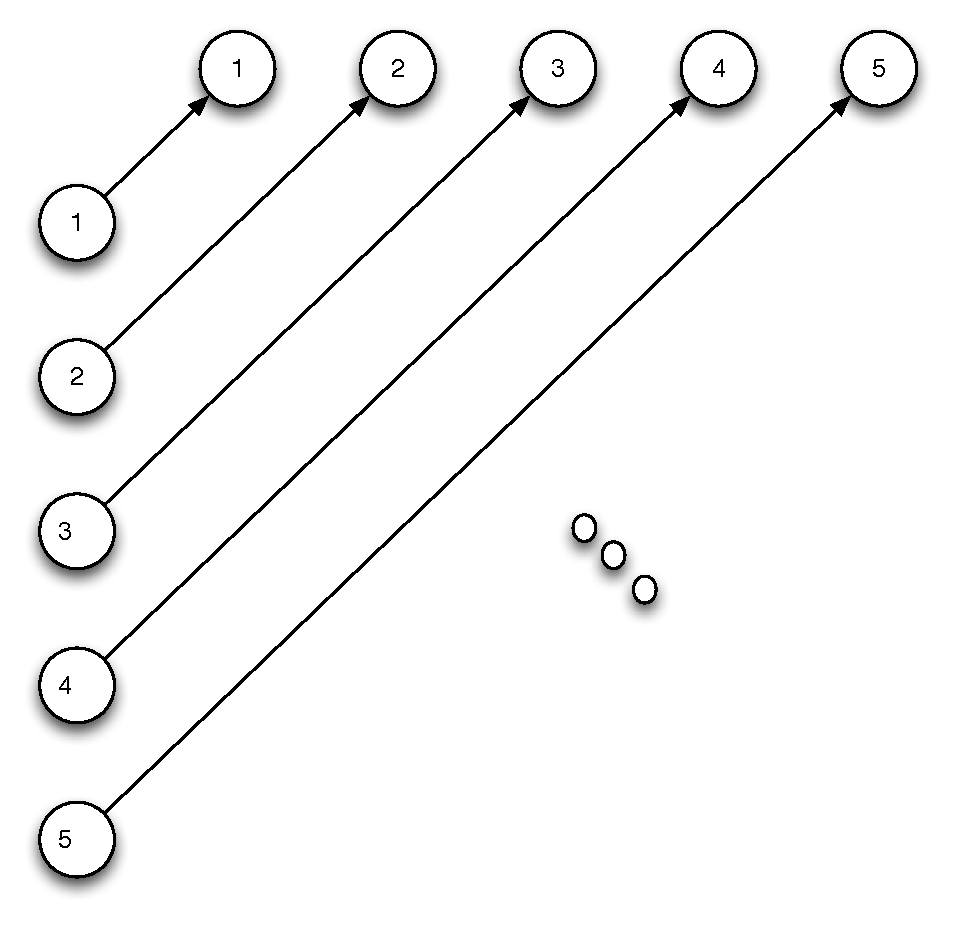
\includegraphics[scale=.5]{problem_1_a.eps}
      \label{fig:problem_1_a}
    \end{figure}
    \noindent Then, if we let each unique pair $(i,j) = a, b, c, \ldots$ we can show a correspondence between those pairs and $k$.\\
    See figure ~\ref{fig:problem_1_b}.
    \begin{figure}[H]
      \centering
      \caption{$f: \mathbb{N} \times \mathbb{N} \rightarrow \mathbb{N}$}
      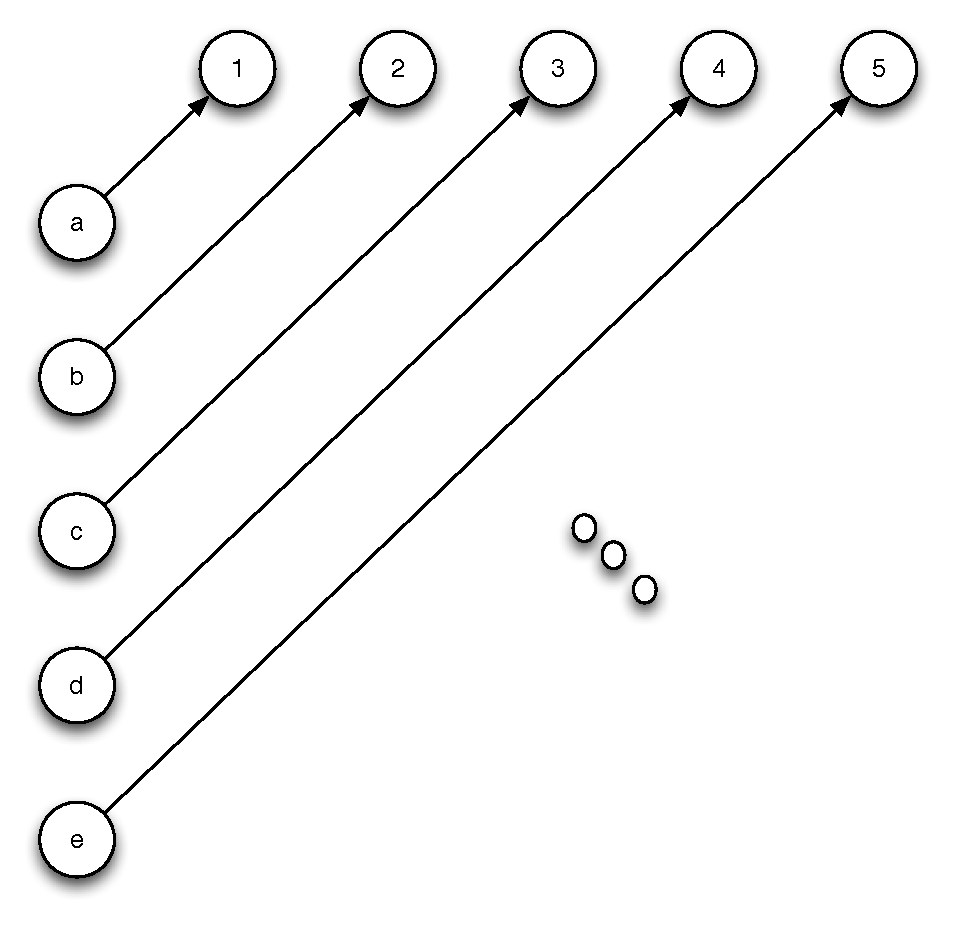
\includegraphics[scale=.5]{problem_1_b.eps}
      \label{fig:problem_1_b}
    \end{figure}
    Because $T$ is onto and one-to-one with $\mathbb{N}$ we can show that these sets are the same size and thus are
    countable.
  \end{solution}
\end{problem}

\begin{problem}{2}
  Let F be the set of all functions from natural numbers to natural numbers. Using a diagonalization argument, show that
  F is uncountable. Hint: If F is countable, you should be able to list its elements in some order. Use this together
  with a diagonalization argument to derive a contradiction.
\end{problem}

\begin{problem}{3}
  Consider the following language: $S = \{<M> | M \text{ is a DFA that accepts } w^R \text{ whenever it accepts w }\}$. Show that S is
  decidable.
  \begin{solution}
    We need to ensure that the reverse of $M$ is equivalent to $M$. We can construct a Turing machine as follows:
    T = ``On input $\tuple{M}$ where M is a DFA:
    \begin{enumerate}
      \item Create a DFA $M'$ from $M$. Since NFAs and DFAs are equivalent in power we're still maintaining the conditions.\\
      \item Reverse the transition function in $M'$ and make all accept states start states, and vice versa.\\
      \item Ensure there are epsilon transitions so that multiple accept states are now multiple start states.\\
      \item Run $EQ_{DFA}$ (given in the book) on $\tuple{M, DFA(M')}$\\
      \item If $EQ_{DFA}$ accepts, T accepts, if $EQ_{DFA}$ rejects, T rejects.\\
    \end{enumerate}
    ''

    \noindent Since $EQ_{DFA}$ is decidable and decides that $M$ and $M'$ are equal where $M'$ is the reverse of $M$, $S$ is also
    decidable.
  \end{solution}
\end{problem}

\begin{problem}{4}
  Let $C = \{<G,x> | \text{G is a CFG that generates at least one string that has x as a substring}\}$. Show that C is decidable.
  (Hint: Use properties of context-free languages to change the question to be answered in such a way that you can
  invoke the decider for $E_{CFG}$.)
\end{problem}

\begin{problem}{5}
  Let A be a Turing-recognizable language consisting of descriptions of Turing machines $\{<M_1>, <M_2>,...\}$, where
  every $M_i$ is a decider. Prove that some decidable language D is not decided by any decider $M_j$ whose description
  appears in A. (Hint: you may find it helpful to consider an enumerator for A.)
\end{problem}

\begin{problem}{6}
  Let C be a language. Prove that C is Turing-recognizable if and only if a decidable language D exists such that $C =
  \{x | \exists y <x,y> \in D\}$. (Hint: For any fixed $n$, is it decidable if a Turing machine accepts a string in (at
  most) $n$ steps?)
\end{problem}

\begin{problem}{7 (EC)}
  Consider the language $HALT_{TM} = \{<M,w> | M \text{ is a Turing machine and M halts on w} \}$. We will see that this
  language is not decidable. However, suppose that we are able to somehow provide a decider for this language. (This
  kind of ``magical'' decider is sometimes called an oracle.) Show that we would then be able to provide a decider for
  the language $D = \{<p> | p \text{ s a diophantine equation with integer roots}\}$.
\end{problem}

\end{document}
